
\de{ĐỀ THI GIỮA HỌC KỲ II NĂM HỌC 2022-2023}{THPT Nguyễn Thị Minh Khai}


%%%% Bài 1
\begin{bt}%[0T7B3-2]%[Dự án đề kiểm tra GKII NH22-23 - Thành Đức Trung]%[THPT Nguyễn Thị Minh Khai - Hồ Chí Minh]
Giải các phương trình
\begin{enumerate}
\item $\sqrt{2x^2-10x-3}=2-x$.
\item $\sqrt{x^2-2x-2}=\sqrt{3x-8}$.
\end{enumerate}
\loigiai{
\begin{enumerate}
\item Ta có 
\begin{align*}
\sqrt{2x^2-10x-3}=2-x&\Leftrightarrow \heva{&2-x\geq 0\\&2x^2-10x-3=(2-x)^2}\\&\Leftrightarrow\heva{&x\leq 2\\& x^2-6x-7=0}\\&\Leftrightarrow\heva{&x\leq 2\\& \hoac{&x=-1\\&x=7}}\\&\Leftrightarrow x =-1.
\end{align*}
Vậy phương trình có một nghiệm.
\item Ta có 
\begin{align*}
\sqrt{x^2-2x-2}=\sqrt{3x-8}&\Leftrightarrow x^2-2x-2=3x-8\\&\Leftrightarrow x^2-5x+6=0\\&\Leftrightarrow \hoac{&x=2\\&x=3.}
\end{align*}
Thử lại ta thấy $x=3$ thỏa mãn yêu cầu bài toán.
\end{enumerate}
}
\end{bt}

%%%% Bài 2
\begin{bt}%[0T7B2-2]%[Dự án đề kiểm tra GHKII NH22-23 - Thành Đức Trung]%[THPT Nguyễn Thị Minh Khai]
\immini
{Sau khi được ném lên, độ cao $y$ (mét) của một quả bóng so với mặt đất sau $x$ (giây) được cho bởi hàm số $y(x)=-0{,}02x^2+0{,}4x$. Hỏi quả bóng đạt độ cao lớn hơn $1{,}5$ (mét) so với mặt đất trong thời gian khoảng bao lâu?
}
{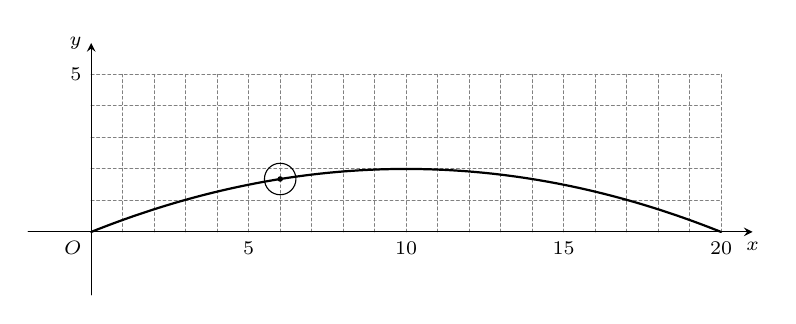
\begin{tikzpicture}[scale=0.4, font=\footnotesize, line join=round, line cap=round, >=stealth]
\def\a{-0.02}
\def\b{0.4}
\def\c{0}
\draw[color=gray,dash pattern=on 1pt off 1pt,xstep=1.0cm,ystep=1.0cm] (0,0) grid (20,5);
\draw[->] (-2,0)--(21,0) node[below] {\scriptsize $x$};
\draw[->] (0,-2)--(0,6) node[left] {\scriptsize $y$};
\draw (0,0)node[below left]{\scriptsize $O$};
\draw (5,0)node[below]{\scriptsize $5$};
\draw (10,0)node[below]{\scriptsize $10$};
\draw (15,0)node[below]{\scriptsize $15$};
\draw (20,0)node[below]{\scriptsize $20$};
\draw[thick,samples=150,smooth,domain=0:20] plot(\x,{\a*(\x)^2+(\b)*\x+(\c)});
\draw (0,5) node[left]{\scriptsize $5$};
\draw (6,1.68) circle[radius=0.5cm];
\draw[fill=black] (6,1.68) circle(2pt);
\end{tikzpicture}
}
\loigiai{
Để độ cao quả bóng cao hơn $1{,}5$ (mét) thì
\[y>1,5\Leftrightarrow-0{,}02x^2+0{,}4x>1{,}5\Leftrightarrow x^2-20x+75<0\Leftrightarrow (x-5)(x-15)<0\Leftrightarrow 5<x<15.\]
Khoảng thời gian độ cao quả bóng lớn hơn $1{,}5$ (mét) so với mặt đất là $15-5=10$ (giây).
}
\end{bt}

%%%% Bài 3
\begin{bt}%[0T7B2-1]%[Dự án đề kiểm tra GHKII NH22-23 - Thành Đức Trung]%[THPT Nguyễn Thị Minh Khai]
Cho biểu thức $f(x)=(m+1)x^2-2(m-1)x+3m-3$. Tìm tất cả các giá trị của tham số $m$ sao cho $f(x)\le0$; $\forall x\in\mathbb{R}$.
\loigiai{
\textbf{Trường hợp 1:} Nếu $m=-1$, khi đó $f(x)=4x-6$, $f(x)\le0\Leftrightarrow x\le\dfrac{3}{2}$ (loại).\\
\textbf{Trường hợp 2:} Nếu $m\ne-1$, để $f(x)\le0$ với mọi $x\in\mathbb{R}$ thì
\[\heva{&m+1<0\\&\Delta'=(m-1)^2-(m+1)(3m-3)\le0}\Leftrightarrow\heva{&m<-1\\&-2m^2-2m+4\le0}\Leftrightarrow\Leftrightarrow\heva{&m<-1\\&\hoac{&m\ge1\\&m\le-2}}\Leftrightarrow m\le-2.\]
Vậy tất cả các giá trị của $m$ thoả mãn yêu cầu bài toán là $m\le-2$.
}
\end{bt}


%%%% Bài 1
\begin{bt}%[0T7B3-2]%[Dự án đề kiểm tra GKII NH22-23 - Thành Đức Trung]%[THPT Nguyễn Thị Minh Khai - Hồ Chí Minh]
Giải các phương trình
\begin{enumerate}
\item $\sqrt{2x^2-10x-3}=2-x$.
\item $\sqrt{x^2-2x-2}=\sqrt{3x-8}$.
\end{enumerate}
\loigiai{
\begin{enumerate}
\item Ta có 
\begin{align*}
\sqrt{2x^2-10x-3}=2-x&\Leftrightarrow \heva{&2-x\geq 0\\&2x^2-10x-3=(2-x)^2}\\&\Leftrightarrow\heva{&x\leq 2\\& x^2-6x-7=0}\\&\Leftrightarrow\heva{&x\leq 2\\& \hoac{&x=-1\\&x=7}}\\&\Leftrightarrow x =-1.
\end{align*}
Vậy phương trình có một nghiệm.
\item Ta có 
\begin{align*}
\sqrt{x^2-2x-2}=\sqrt{3x-8}&\Leftrightarrow x^2-2x-2=3x-8\\&\Leftrightarrow x^2-5x+6=0\\&\Leftrightarrow \hoac{&x=2\\&x=3.}
\end{align*}
Thử lại ta thấy $x=3$ thỏa mãn yêu cầu bài toán.
\end{enumerate}
}
\end{bt}

%%%% Bài 2
\begin{bt}%[0T7B2-2]%[Dự án đề kiểm tra GHKII NH22-23 - Thành Đức Trung]%[THPT Nguyễn Thị Minh Khai]
\immini
{Sau khi được ném lên, độ cao $y$ (mét) của một quả bóng so với mặt đất sau $x$ (giây) được cho bởi hàm số $y(x)=-0{,}02x^2+0{,}4x$. Hỏi quả bóng đạt độ cao lớn hơn $1{,}5$ (mét) so với mặt đất trong thời gian khoảng bao lâu?
}
{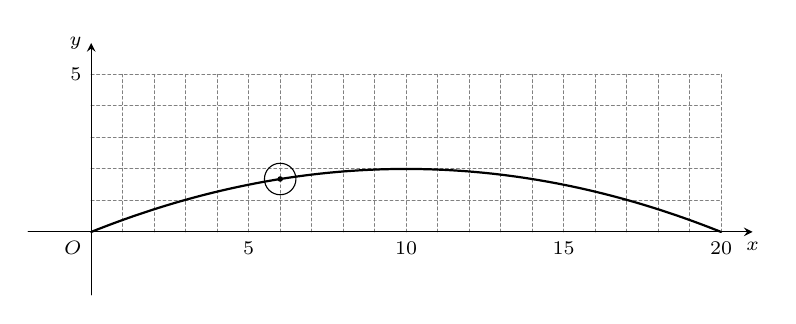
\begin{tikzpicture}[scale=0.4, font=\footnotesize, line join=round, line cap=round, >=stealth]
\def\a{-0.02}
\def\b{0.4}
\def\c{0}
\draw[color=gray,dash pattern=on 1pt off 1pt,xstep=1.0cm,ystep=1.0cm] (0,0) grid (20,5);
\draw[->] (-2,0)--(21,0) node[below] {\scriptsize $x$};
\draw[->] (0,-2)--(0,6) node[left] {\scriptsize $y$};
\draw (0,0)node[below left]{\scriptsize $O$};
\draw (5,0)node[below]{\scriptsize $5$};
\draw (10,0)node[below]{\scriptsize $10$};
\draw (15,0)node[below]{\scriptsize $15$};
\draw (20,0)node[below]{\scriptsize $20$};
\draw[thick,samples=150,smooth,domain=0:20] plot(\x,{\a*(\x)^2+(\b)*\x+(\c)});
\draw (0,5) node[left]{\scriptsize $5$};
\draw (6,1.68) circle[radius=0.5cm];
\draw[fill=black] (6,1.68) circle(2pt);
\end{tikzpicture}
}
\loigiai{
Để độ cao quả bóng cao hơn $1{,}5$ (mét) thì
\[y>1,5\Leftrightarrow-0{,}02x^2+0{,}4x>1{,}5\Leftrightarrow x^2-20x+75<0\Leftrightarrow (x-5)(x-15)<0\Leftrightarrow 5<x<15.\]
Khoảng thời gian độ cao quả bóng lớn hơn $1{,}5$ (mét) so với mặt đất là $15-5=10$ (giây).
}
\end{bt}

%%%% Bài 3
\begin{bt}%[0T7B2-1]%[Dự án đề kiểm tra GHKII NH22-23 - Thành Đức Trung]%[THPT Nguyễn Thị Minh Khai]
Cho biểu thức $f(x)=(m+1)x^2-2(m-1)x+3m-3$. Tìm tất cả các giá trị của tham số $m$ sao cho $f(x)\le0$; $\forall x\in\mathbb{R}$.
\loigiai{
\textbf{Trường hợp 1:} Nếu $m=-1$, khi đó $f(x)=4x-6$, $f(x)\le0\Leftrightarrow x\le\dfrac{3}{2}$ (loại).\\
\textbf{Trường hợp 2:} Nếu $m\ne-1$, để $f(x)\le0$ với mọi $x\in\mathbb{R}$ thì
\[\heva{&m+1<0\\&\Delta'=(m-1)^2-(m+1)(3m-3)\le0}\Leftrightarrow\heva{&m<-1\\&-2m^2-2m+4\le0}\Leftrightarrow\Leftrightarrow\heva{&m<-1\\&\hoac{&m\ge1\\&m\le-2}}\Leftrightarrow m\le-2.\]
Vậy tất cả các giá trị của $m$ thoả mãn yêu cầu bài toán là $m\le-2$.
}
\end{bt}


\begin{bt}%[0T9B1-3]%%[Trường Nguyễn Minh Khai][Dự án đề kiểm tra HKII NH22-23-Nguyễn Tài Tuệ] 
	Trong mặt phẳng $Oxy$, cho $\triangle ABC$ với $A(1;-2)$, $B(2 ; 0)$, $C(7 ;-5)$.
 \begin{enumerate}
 	\item Chứng minh $\triangle ABC$ vuông tại $A$.
 	\item Tìm tọa độ điểm $D$ sao cho tứ giác $ABCD$ là hình bình hành.
 \end{enumerate}
\loigiai{
	\begin{enumerate}
		\item Ta có $ \overrightarrow{AB} =(1;2) $, $ \overrightarrow{AC}=(6;-3)$.\\
		Ta có $ \vec{AB}\cdot \vec{AC} =1\cdot 6+2\cdot (-3)=0 $.\\
		Do đó $ AB\perp AC $, hay tam giác $ ABC $ vuông tại $ A $.
		\item Gọi $ D(x;y) $, ta có $ \vec{DC}=(7-x; -5-y) $.\\
		Mà $ A $, $ B $, $ C $ là ba đỉnh của tam giác nên $ ABCD $ là hình bình hành khi và chỉ khi $$\vec{AB}=\vec{DC}\Leftrightarrow \heva{&1=7-x\\&2=-5-y}\Leftrightarrow \heva{& x=6\\&y=-7.} $$
		Vậy $ D(6;-7) $.
	\end{enumerate}
	
}
\end{bt}
\begin{bt}%[0T9K2-5]%[Trường Nguyễn Minh Khai][Dự án đề kiểm tra HKII NH22-23-Nguyễn Tài Tuệ] 
  Trong mặt phẳng $Oxy$, cho đường thẳng $(\Delta)\colon x-2 y+2023=0$ và hai điểm $P(2; 5)$, $Q(5; 1)$.
\begin{enumerate}
	\item Viết phương trình đường thẳng $\left(d_1\right)$ đi qua điểm $P$ và song song với đường thẳng $(\Delta)$.
	\item Viết phương trình đường thẳng $\left(d_2\right)$ đi qua điểm $P$ và cách điểm $Q$ một khoảng bằng $  3  $.
\end{enumerate}  
   \loigiai{
   	\begin{enumerate}
   		\item Đường thẳng $ (d_1) $ song song với đường thẳng $ (\Delta) $ nên đường thẳng $ (d_1) $ có dạng $ x-2y+c=0 $, với $ c\ne 2023 $.\\
   		Mà $ P\in (d_1) $ nên $2-2\cdot 5+c=0 \Leftrightarrow c=8$.\\
   		Vậy phương trình đường thẳng $ d_1\colon x-2y+8=0 $.
   		\item Gọi $ \vec{n}(a;b) $ là một véc-tơ pháp tuyến của đường thẳng $ d_2 $, với $ a^2+b^2\ne 0 $.\\
   		Phương trình đường thẳng $ d_2 $ có dạng $ a(x-2)+b(y-5)=0 \Leftrightarrow ax+by-2a-5b=0$.\\
   		Ta có
   		\begin{eqnarray*}
   			&& \mathrm{d}(Q,(d_2)) =3\\
   			&\Leftrightarrow& \dfrac{|5a+b-2a-5b|}{\sqrt{a^2+b^2}}=3\\
   			&\Leftrightarrow& |3a-4b|=3\sqrt{a^2+b^2} \\
   			&\Leftrightarrow& 9a^2 -24ab+16b^2 =9(a^2+b^2) \\
   			&\Leftrightarrow& 7b^2-24ab =0\\
   			&\Leftrightarrow& \hoac{&b=0\\&7b-24a=0.}
   		\end{eqnarray*}  
   		\begin{itemize}
   			\item Với $b=0$, chọn $a=1$, suy ra phương trình đường thẳng $d_2\colon x-2=0$.
   			\item Với $ 7b-24a=0 $, chọn $ a=7, b=24 $, suy ra phương trình đường thẳng $$ d_2\colon 7x+24y-134=0.$$
   		\end{itemize}
   	\end{enumerate}
   }
\end{bt}
 

